\documentclass{article}

\usepackage[latin1]{inputenc}
\usepackage{pgfplots}
\usepackage{tikz}

\pgfplotsset{compat=1.10}

% GNUPLOT required
\begin{document}
\pagestyle{empty}

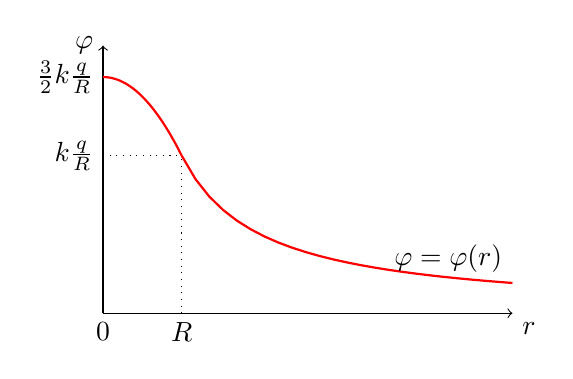
\begin{tikzpicture}
	%axes
	\draw[->] (0,0) -- (5.2,0) node[below right] {$r$};
	\draw[->] (0,0) -- (0,3.4) node[left] {$\varphi$};

	\node[below] at (0, 0) {$0$};
	\node[left] at (0, 3) {$\frac{3}{2}k\frac{q}{R}$};
	\node[left] at (0, 2) {$k\frac{q}{R}$};
	\node[below] at (1, 0) {$R$};
	\draw[thin, dotted] (1, 0) -- (1, 2);
	\draw[thin, dotted] (0, 2) -- (1, 2);

	%plot
	\draw[red, thick, domain=0:1] plot (\x, {-\x*\x+3});
    \draw[red, thick, domain=1:5.2] plot (\x, {2/\x}) node[black, above left] {$\varphi=\varphi(r)$};
\end{tikzpicture}


\end{document}